\subsection{Initial Results}
\begin{frame}
  \frametitle{Model Flow}
  \begin{enumerate}
    \item Start with randomly chosen hyperparameters
    \item Predicting a single quantity (e.g. energy generation)
    \item Set the prediction window to 72-hours in the future
    \item Optimize with a hyper-parameter grid search
  \end{enumerate}
\end{frame}

\begin{frame}
  \frametitle{Solar Prediction}
  \begin{figure}
  \centering
  \begin{tabular}{@{}c@{}}
    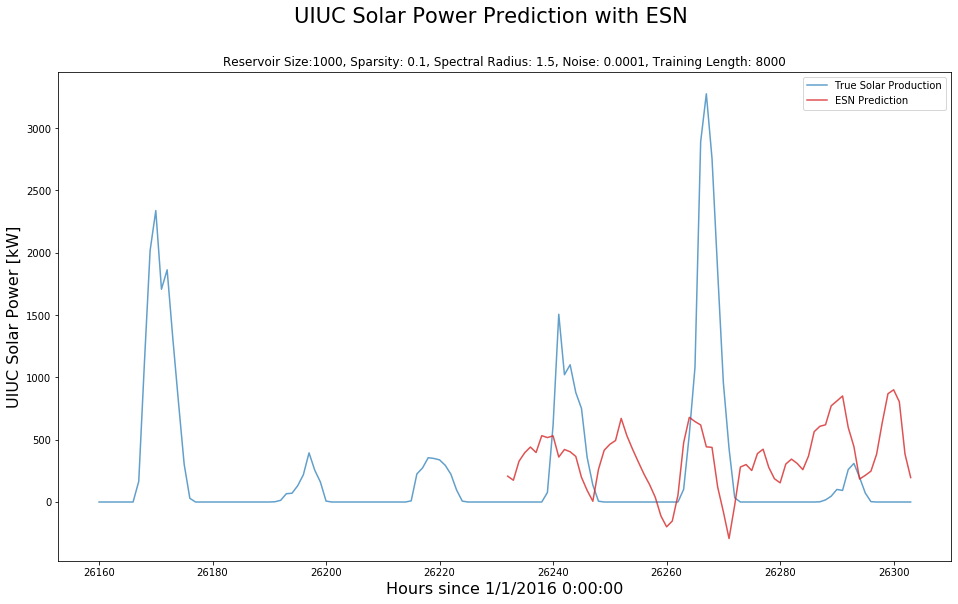
\includegraphics[width=0.45\textwidth]{solarpower01.png}
  \end{tabular}

  \begin{tabular}{@{}c@{}}
    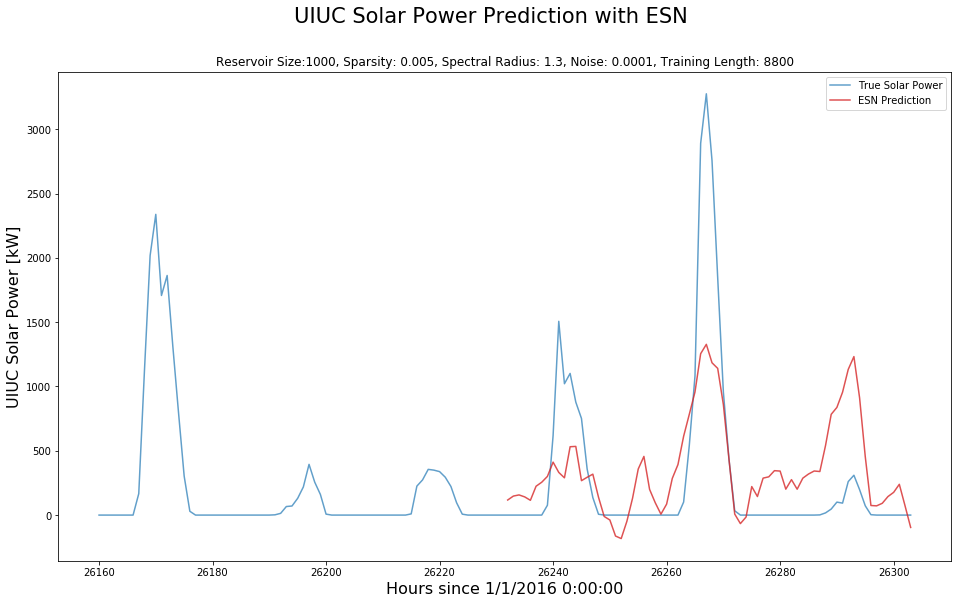
\includegraphics[width=0.45\textwidth]{solarpower02.png}
  \end{tabular}

  \caption{Top: Prediction with random hyperparameters. Bottom: Prediction with optimized hyperparameters.}\label{fig:myfig}
\end{figure}
\end{frame}

\begin{frame}
  \frametitle{Wind Prediction}
  \begin{figure}
  \centering
  \begin{tabular}{@{}c@{}}
    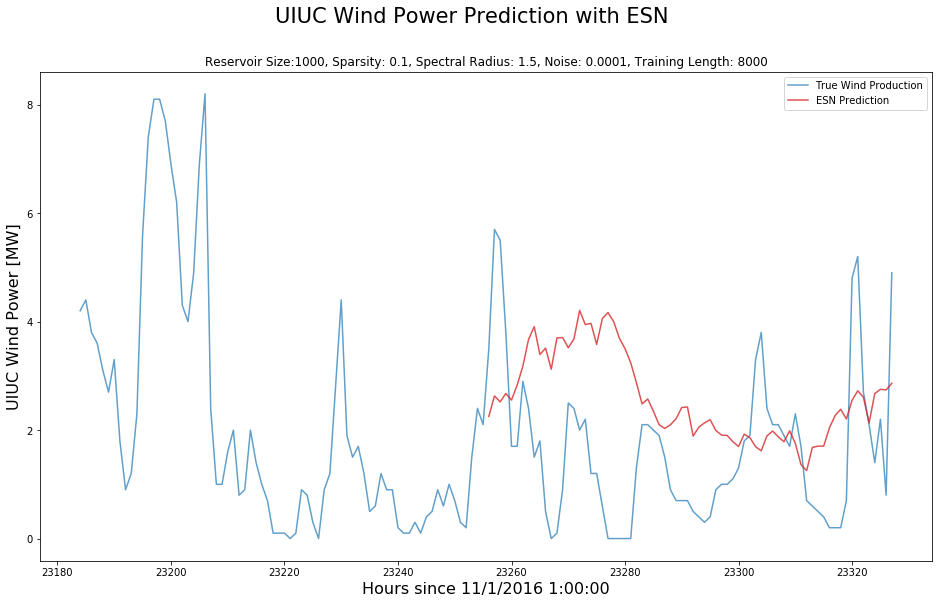
\includegraphics[width=0.45\textwidth]{windpower01.png}
  \end{tabular}

  \begin{tabular}{@{}c@{}}
    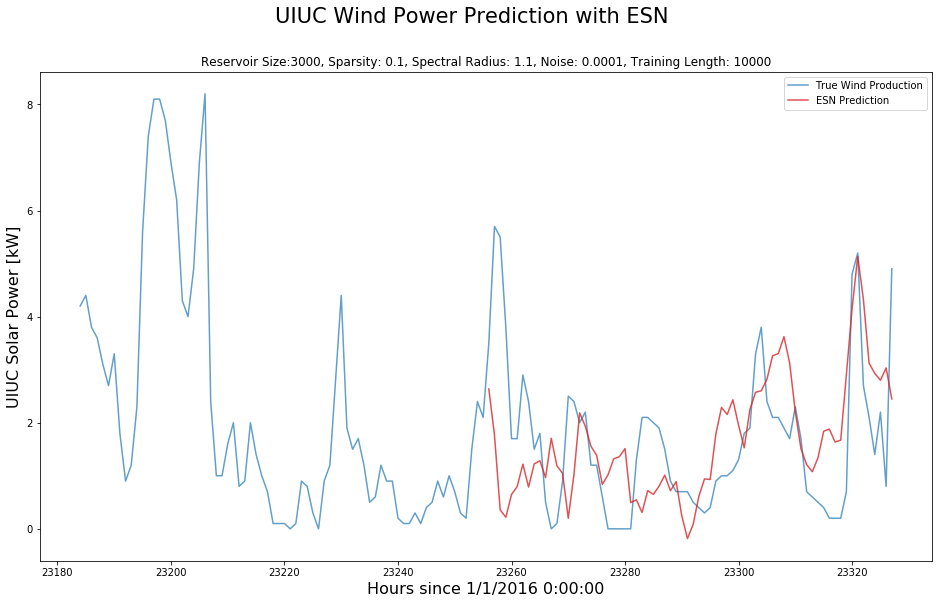
\includegraphics[width=0.45\textwidth]{windpower02.png}
  \end{tabular}

  \caption{Top: Prediction with random hyperparameters. Bottom: Prediction with optimized hyperparameters.}\label{fig:myfig}
\end{figure}
\end{frame}
\begin{frame}
  \frametitle{Total Demand Prediction}
  \begin{figure}
  \centering
  \begin{tabular}{@{}c@{}}
    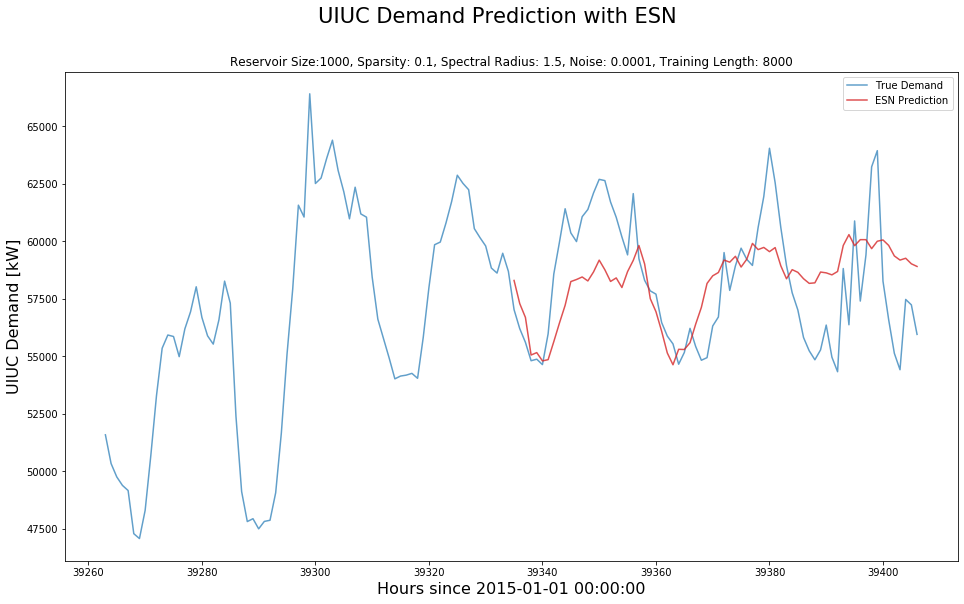
\includegraphics[width=0.45\textwidth]{demand01.png}
  \end{tabular}

  \begin{tabular}{@{}c@{}}
    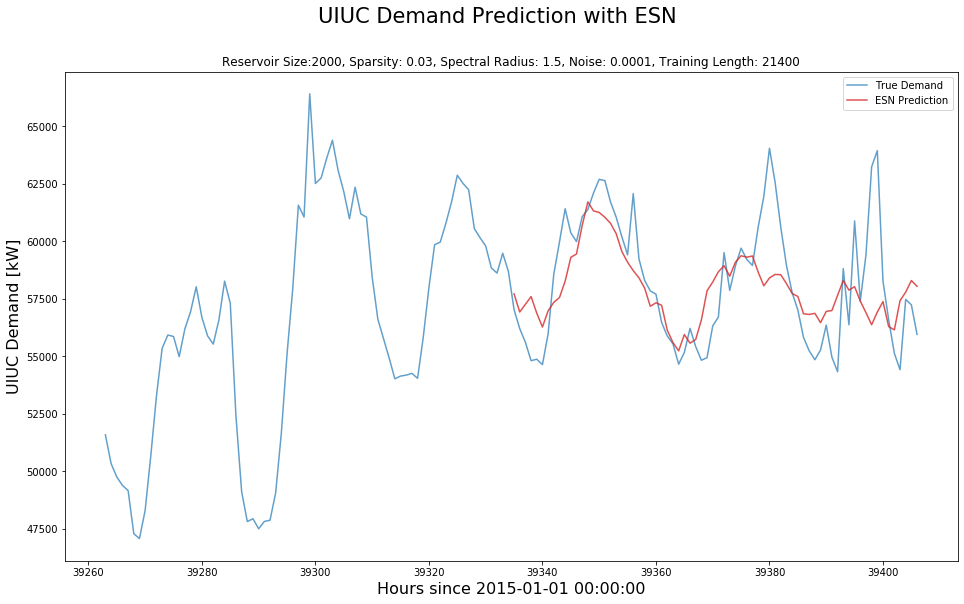
\includegraphics[width=0.45\textwidth]{demand02.png}
  \end{tabular}

  \caption{Top: Prediction with random hyperparameters. Bottom: Prediction with optimized hyperparameters.}\label{fig:myfig}
\end{figure}
\end{frame}
\begin{frame}
  \frametitle{Net Demand Prediction}
  \begin{figure}
  \centering
  \begin{tabular}{@{}c@{}}
    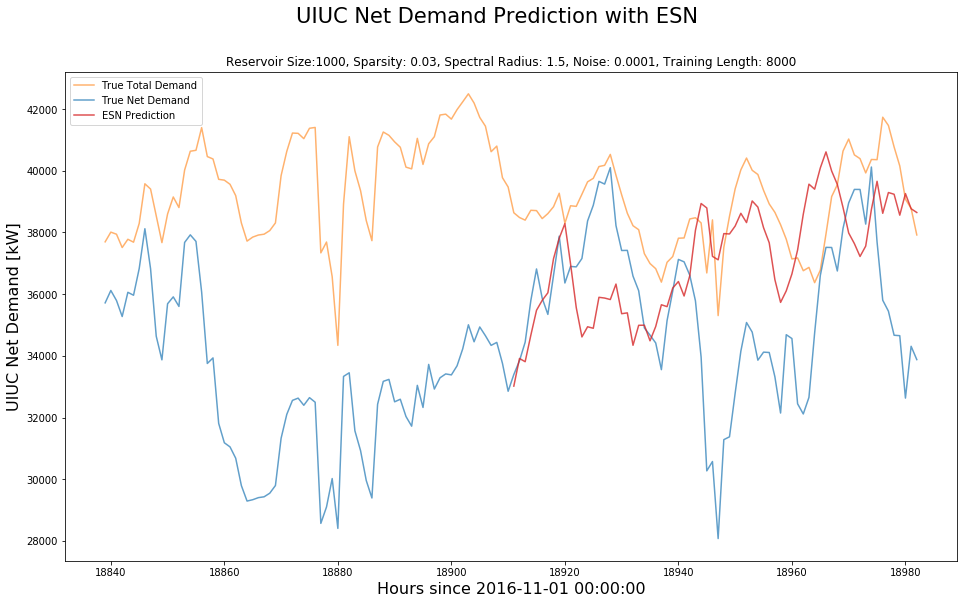
\includegraphics[width=0.45\textwidth]{netdem_01.png}
  \end{tabular}

  \begin{tabular}{@{}c@{}}
    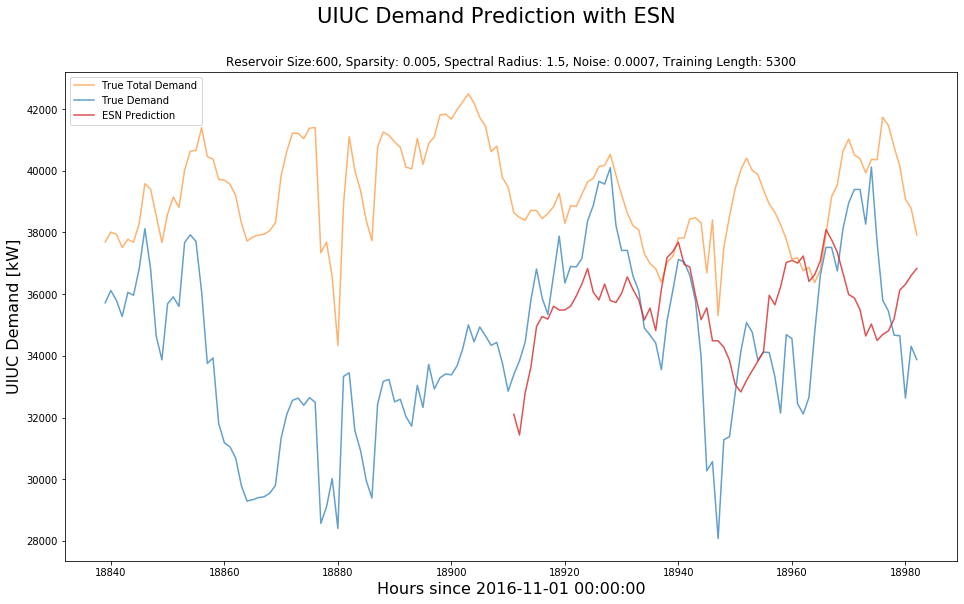
\includegraphics[width=0.45\textwidth]{netdem_02.png}
  \end{tabular}

  \caption{Top: Prediction with random hyperparameters. Bottom: Prediction with optimized hyperparameters.}\label{fig:myfig}
\end{figure}
\end{frame}

\subsection{Improving the Model}
\begin{frame}
  \frametitle{Model Flow}
  \begin{enumerate}
    \item Start with randomly chosen hyperparameters
    \item \textbf{\textit{Predicting coupled quantities (e.g. energy generation and sun elevation.)}}
    \item Set the prediction window to 72-hours in the future
    \item Optimize with a hyper-parameter grid search
  \end{enumerate}
\end{frame}

\begin{frame}
  \frametitle{Wind Prediction}
  \begin{figure}
  \centering
  \begin{tabular}{@{}c@{}}
    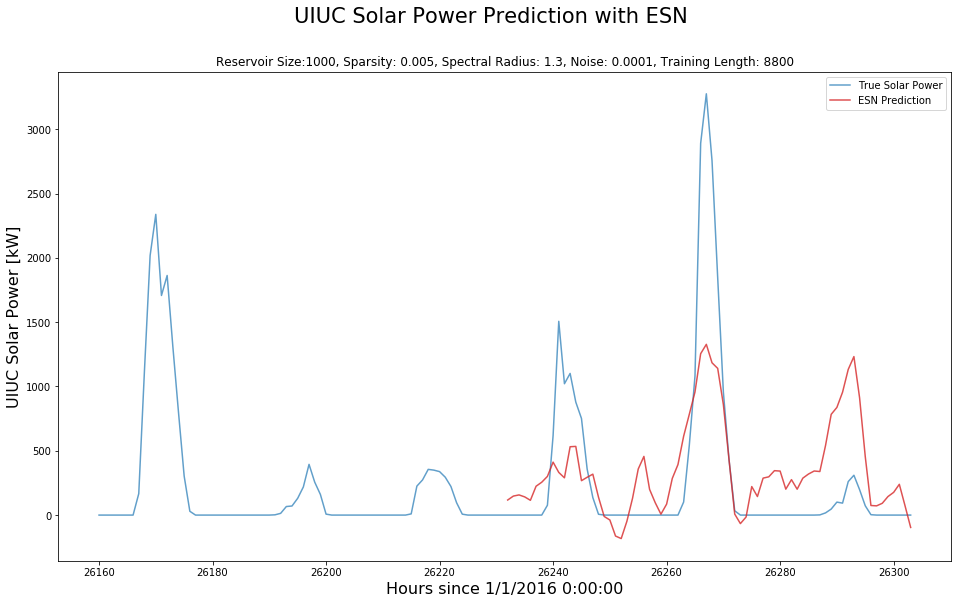
\includegraphics[width=0.45\textwidth]{solarpower02.png}
  \end{tabular}

  \begin{tabular}{@{}c@{}}
    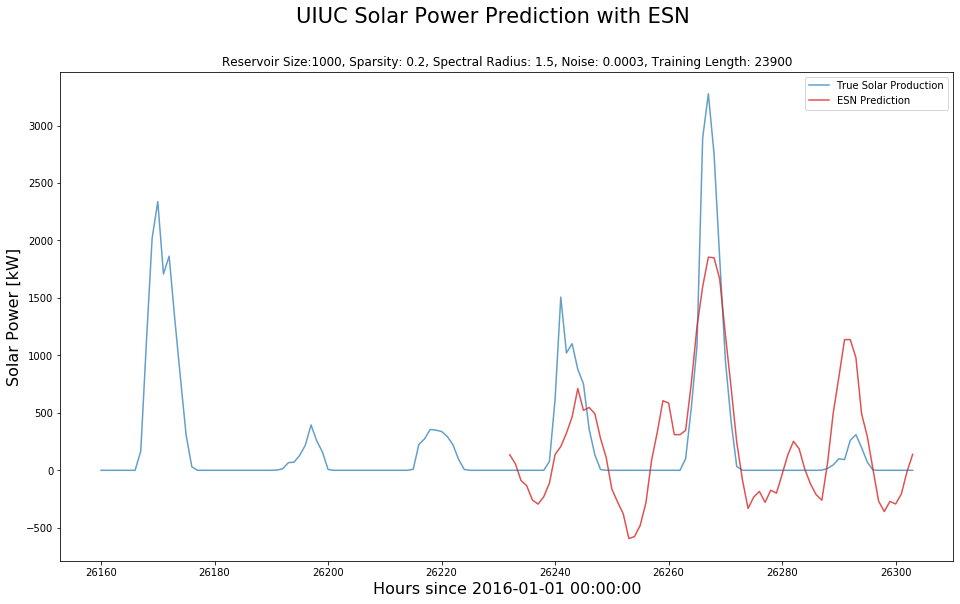
\includegraphics[width=0.45\textwidth]{solarpower-angle02.png}
  \end{tabular}

  \caption{Top: Predicting solar generation alone. Bottom: Predicting solar generation with solar elevation.}\label{fig:myfig}
\end{figure}
\end{frame}

\begin{frame}
  \frametitle{Wind Power Prediction}
  \begin{figure}
  \centering
  \begin{tabular}{@{}c@{}}
    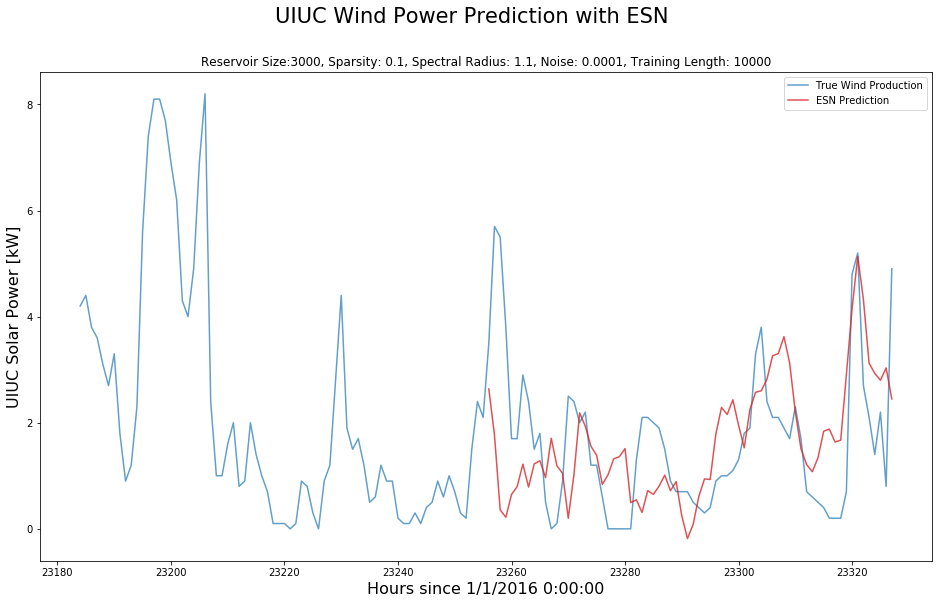
\includegraphics[width=0.45\textwidth]{windpower02.png}
  \end{tabular}

  \begin{tabular}{@{}c@{}}
    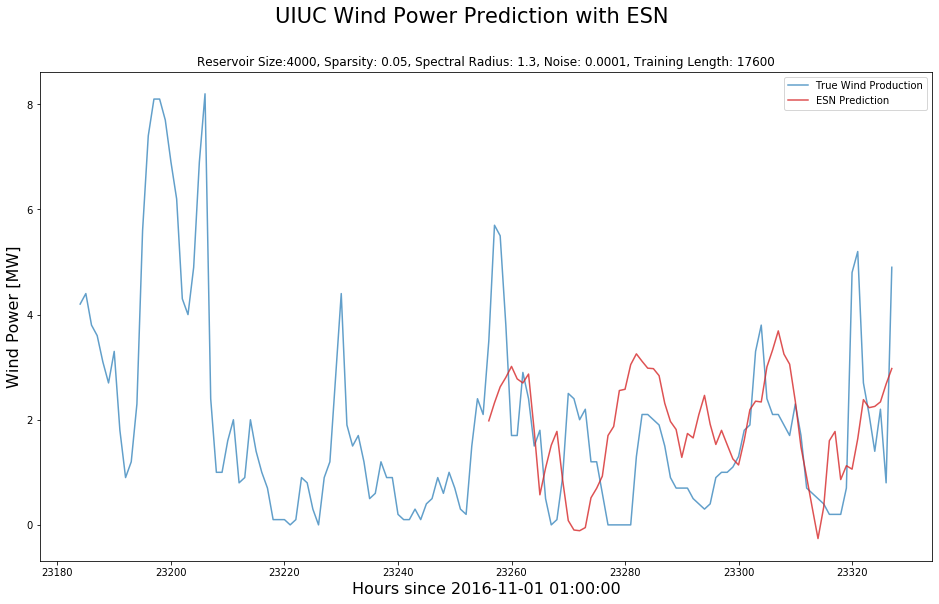
\includegraphics[width=0.45\textwidth]{windpower-angle01.png}
  \end{tabular}

  \caption{Top: Predicting wind generation alone. Bottom: Predicting wind generation with solar elevation.}\label{fig:myfig}
\end{figure}
\end{frame}

\begin{frame}
  \frametitle{Total Demand Prediction}
  \begin{figure}
  \centering
  \begin{tabular}{@{}c@{}}
    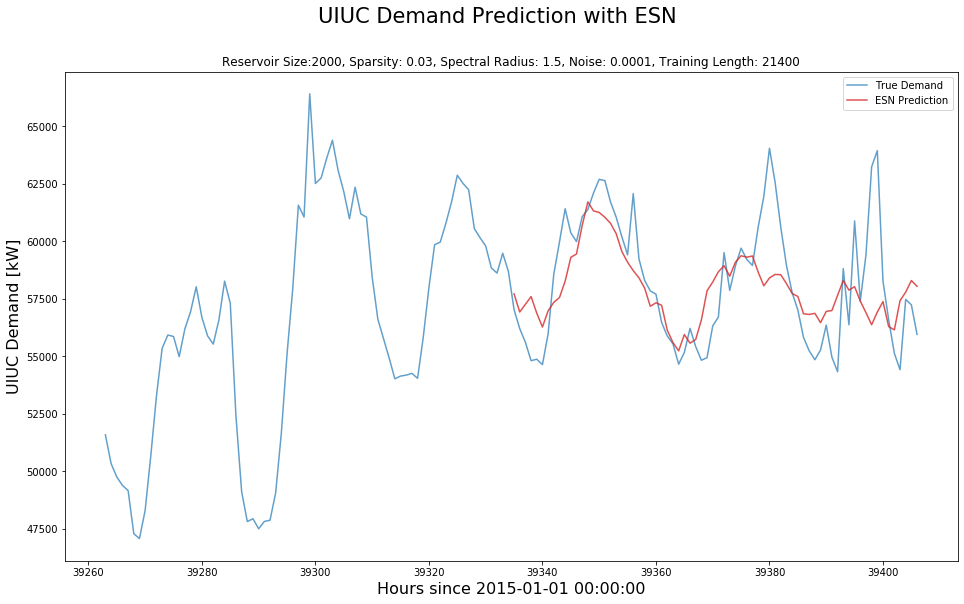
\includegraphics[width=0.45\textwidth]{demand02.png}
  \end{tabular}

  \begin{tabular}{@{}c@{}}
    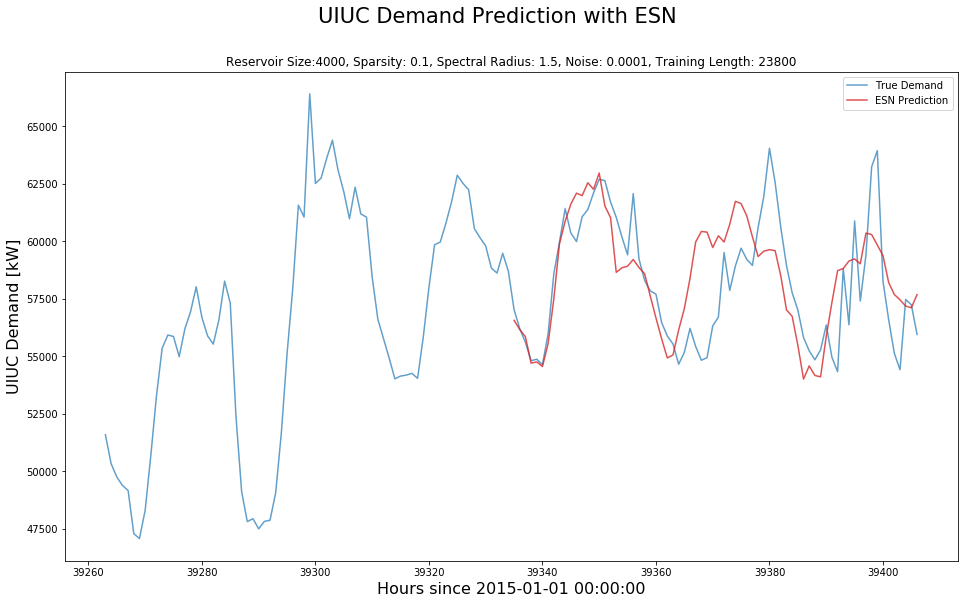
\includegraphics[width=0.45\textwidth]{demsol02.png}
  \end{tabular}

  \caption{Top: Predicting total demand alone. Bottom: Predicting total demand with solar elevation.}\label{fig:myfig}
\end{figure}
\end{frame}

\begin{frame}
  \frametitle{Net Demand Prediction}
  \begin{figure}
  \centering
  \begin{tabular}{@{}c@{}}
    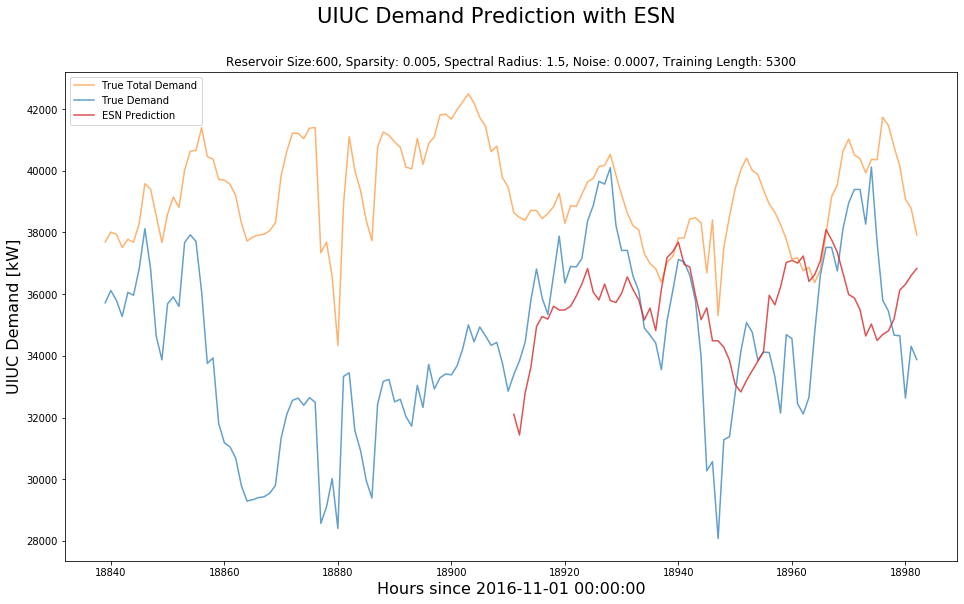
\includegraphics[width=0.45\textwidth]{netdem_02.png}
  \end{tabular}

  \begin{tabular}{@{}c@{}}
    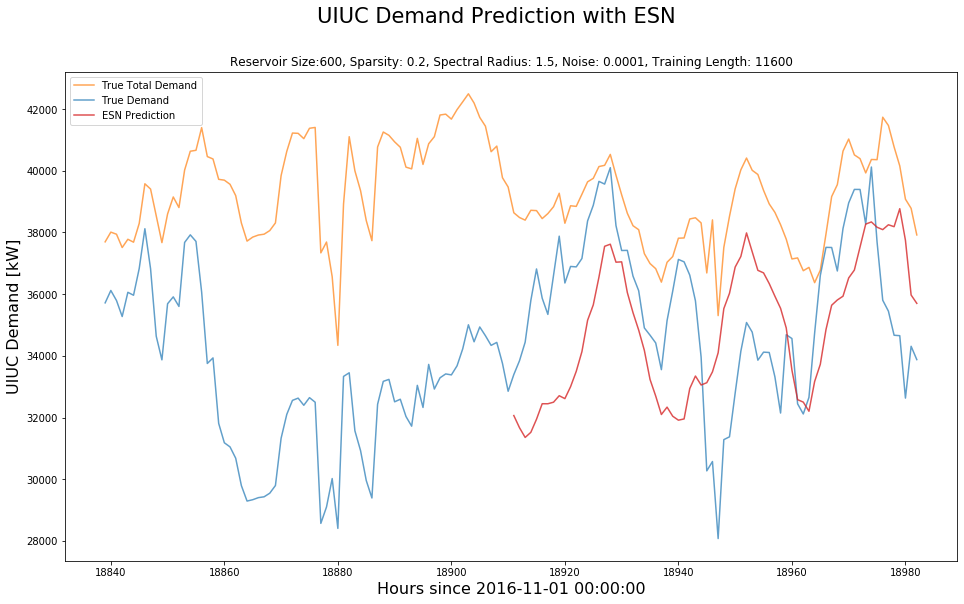
\includegraphics[width=0.45\textwidth]{net_demsol02.png}
  \end{tabular}

  \caption{Top: Predicting net demand alone. Bottom: Predicting net demand with solar elevation.}\label{fig:myfig}
\end{figure}
\end{frame}

\subsection{Uncertainty Analysis}
\begin{frame}
  \frametitle{Uncertainty in Total Demand}
  \begin{figure}
    \centering
    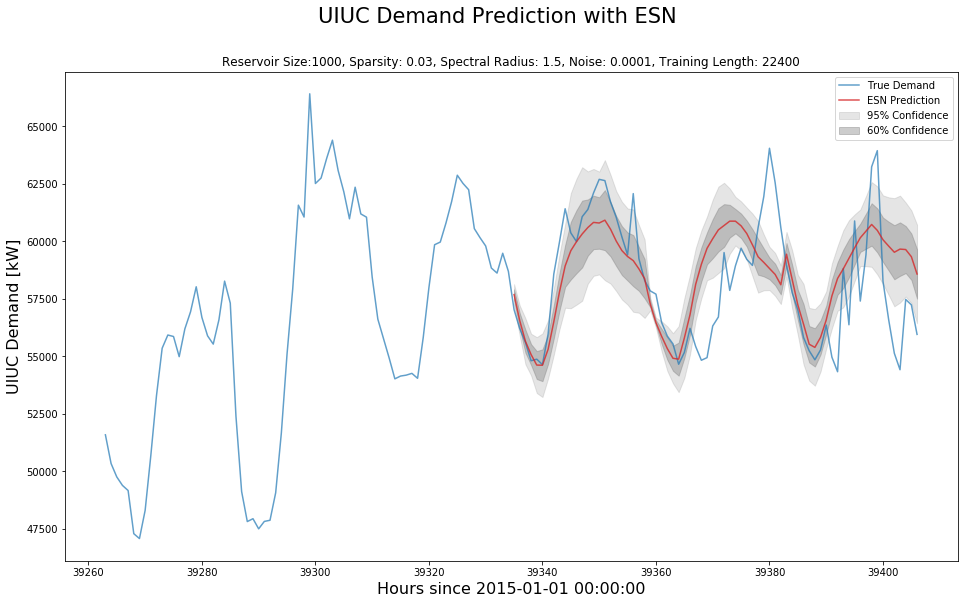
\includegraphics[width=0.85\textwidth]{demsol-bars01.png}
    \caption{Error bars on the prediction for total demand.}
    \label{}
  \end{figure}
\end{frame}
\begin{frame}
  \frametitle{Uncertainty in Net Demand}
  \begin{figure}
    \centering
    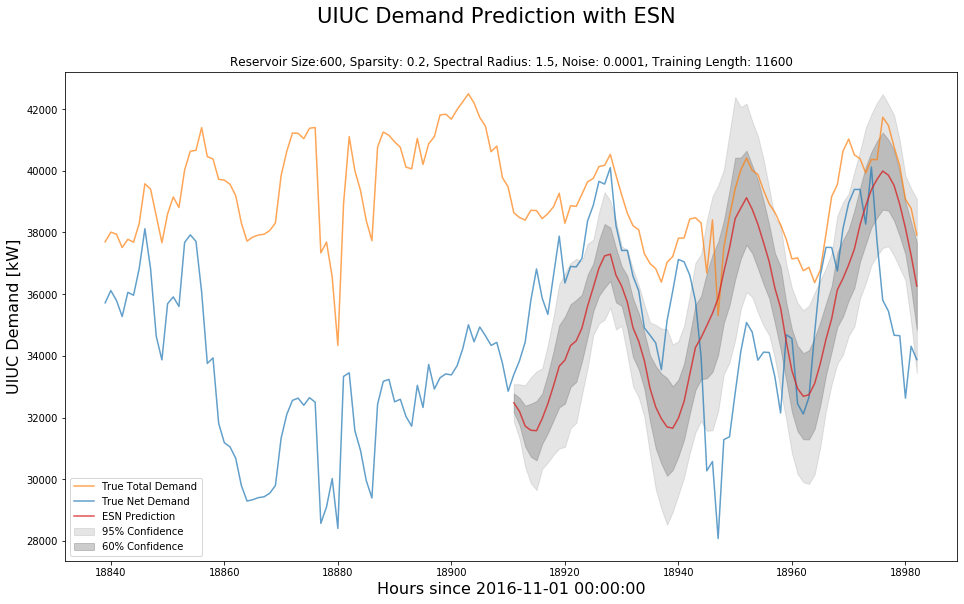
\includegraphics[width=0.85\textwidth]{net_demsol-bars02.png}
    \caption{Error bars on the prediction for net demand.}
    \label{}
  \end{figure}
\end{frame}
\begin{frame}
  \frametitle{Uncertainty in Net Demand -- Very Short Prediction Window}
  \begin{figure}
    \centering
    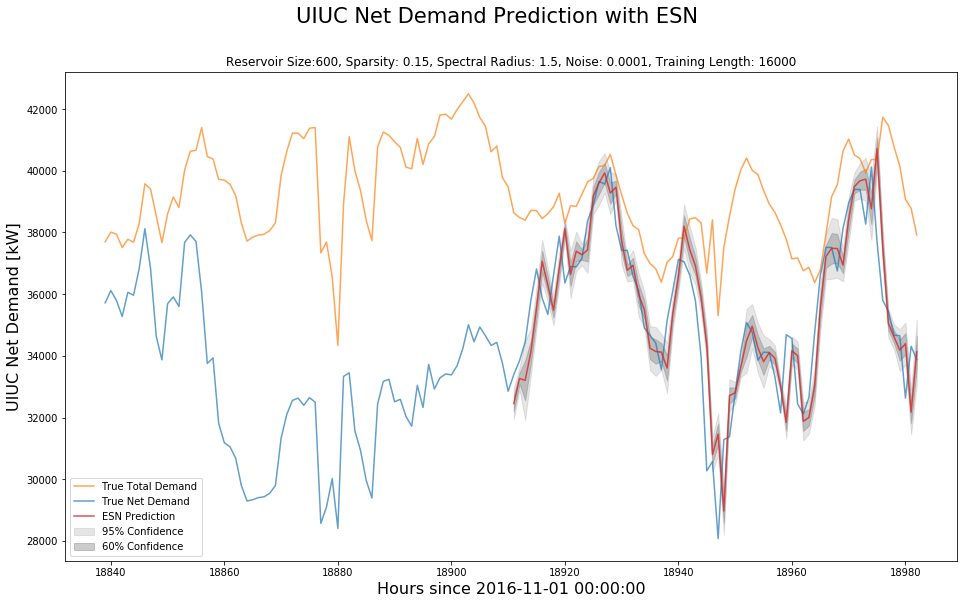
\includegraphics[width=0.85\textwidth]{net_demsol-bars04-1hour.png}
    \caption{Error bars on the prediction for net demand with a prediction window of one hour.}
    \label{}
  \end{figure}
\end{frame}
